\documentclass[tikz,border=6pt]{standalone}
% Shared visual language for the book's standalone vector figures.
% Keep this file compatible with the TeX Live version used by LyX.
\usepackage{amsmath,amssymb}
\usepackage{array,booktabs}
\usepackage{pgfplots}
\usepackage{pgfplotstable}
\usetikzlibrary{arrows.meta,calc,positioning}
\pgfplotsset{compat=1.17}

\definecolor{BookBlue}{HTML}{0072B2}
\definecolor{BookOrange}{HTML}{D55E00}
\definecolor{BookGreen}{HTML}{009E73}
\definecolor{BookGray}{HTML}{666666}
\definecolor{BookLightGray}{HTML}{D9D9D9}

\pgfplotsset{
  book axis/.style={
    axis line style={black!75,line width=0.55pt},
    tick style={black!75,line width=0.45pt},
    tick label style={font=\small},
    label style={font=\small},
    legend style={
      font=\small,
      draw=none,
      fill=none,
      cells={anchor=west},
    },
    grid style={BookLightGray,line width=0.35pt},
    major grid style={BookLightGray,line width=0.35pt},
  },
}

\usepgfplotslibrary{groupplots}
\begin{document}
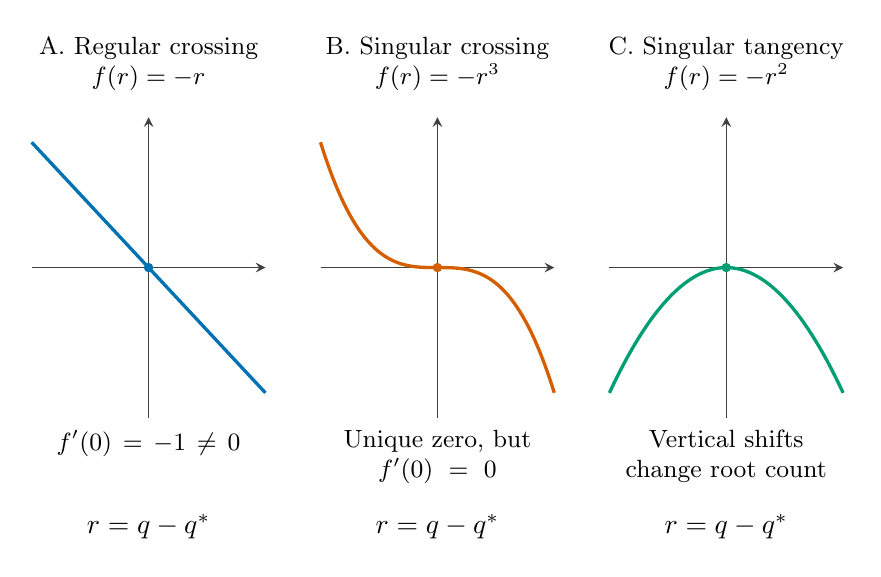
\begin{tikzpicture}
\begin{groupplot}[group style={group size=3 by 1,horizontal sep=.7cm},book axis,
 width=4.55cm,height=5.4cm,xmin=-1,xmax=1,ymin=-1.2,ymax=1.2,
 axis lines=middle,xtick={0},ytick=\empty,xlabel={$r=q-q^*$},
 xlabel style={at={(axis description cs:.5,-.29)},anchor=north},
 title style={font=\small,align=center},clip=false]
 \nextgroupplot[title={A. Regular crossing\\$f(r)=-r$}]
 \addplot[BookBlue,very thick,domain=-1:1]{-x};
 \fill[BookBlue] (axis cs:0,0) circle(1.7pt);
 \node[anchor=north,font=\small,align=center,text width=3cm,
   inner sep=1pt] at(axis description cs:.5,-.03){$f'(0)=-1\ne0$};
 \nextgroupplot[title={B. Singular crossing\\$f(r)=-r^3$}]
 \addplot[BookOrange,very thick,domain=-1:1,samples=100]{-x^3};
 \fill[BookOrange] (axis cs:0,0) circle(1.7pt);
 \node[anchor=north,font=\small,align=center,text width=3cm,
   inner sep=1pt] at(axis description cs:.5,-.03)
   {Unique zero, but\\$f'(0)=0$};
 \nextgroupplot[title={C. Singular tangency\\$f(r)=-r^2$}]
 \addplot[BookGreen,very thick,domain=-1:1,samples=100]{-x^2};
 \fill[BookGreen] (axis cs:0,0) circle(1.7pt);
 \node[anchor=north,font=\small,align=center,text width=3cm,
   inner sep=1pt] at(axis description cs:.5,-.03)
   {Vertical shifts\\change root count};
\end{groupplot}
\end{tikzpicture}
\end{document}
